
\chapter{Modelo clásico}

\label{ch:modelo_clasico}

\section{Introducción}
El modelo que planteamos en esta sección pertenece a el modelado considerado clásico realizado en \cite{schaffer}.

Como tenemos gran parte de la dinámica ya planteada, en esta sección, tal y como avanzamos al principio, vamos a presentar la forma en la que se modela la generación de Gli y Ptc debida a la activación de los genes gli y ptc, modelando precisamente la transcripción genética aplicando un enfoque de métodos de termodinámica estadística.

\section{Modelado BEWARE}
 
 
 
 Partimos de dos resultados experimentales que muestran que gli1, gli2 y ptc están regulados transcripcionalmente por la señalización de Shh.
 
  Definimos $K_1$ como la constante de enlace de disociación de equilibrio de Gli y $K_2$ como la constante de enlace de disociación de equilibrio de $Gli_3$ (tanto activador como represor, Gli3R). Las zonas de unión al ADN de todas las formas de Gli están altamente relacionadas, lo que sugiere que estas las afinidades son similares.
  
  Ante la decisión de qué cantidad de enlaces tomar, \cite{schaffer}, para simplificar, suponen que hay el mismo número de posibles enlaces Gli dentro de los
  promotores para Gli y Ptc.
  
  
  El promotor puede existir en numerosos
  estados posibles (promotor vacío, dos Gli  y un $Gli_3$ y el resto de combinaciones de 3 elementos). Además la probabilidad de cada estado de unión está determinada por las concentraciones relativas de las tres especies (Gli, $Gli_3$, Gli3R) y sus afinidades de unión al ADN. 
  
  
  Nuestro objetivo es desarrollar el modelo de acuerdo al procedimiento BEWARE, por tanto, para modelar el nivel de activación transcripcional del promotor, calculamos la suma de la probabilidad de cada posible estado del promotor multiplicado por una tasa de la activación de transcripción génica que la combinación particular
  induce.
  Sin embargo, para ello debemos determinar correctamente  el nivel de activación para un estado dado, con este fin \cite{schaffer,saha} aplican varias reglas:
   \begin{itemize}
   	 
   
   \item En primer lugar la unión del número máximo de activadores transcripcionales (una combinación de Gli y Gli3) produce un estado con la máxima tasa transcripcional  posible, igual a $(v_{max,G} + r_{bas})$ para el promotor gli.
  
  En este caso $v_{max}$ es la tasa de transcripción inducida máxima y $r_{bas}$ es igual a la tasa basal de transcripción que se obtendría para un promotor completamente independiente.
   Implícita en esta expresión está la suposición de que \cite{schaffer} no tiene en cuenta la dinámica del ARNm, es decir, suponen que cada molécula de ARNm produce un número fijo de proteínas. 
   
   
  \item A continuación, se permite la posibilidad de unión cooperativa de proteínas al promotor, de forma que el promotor con uno o más factores unidos tuviera una afinidad incrementada para el siguiente factor. A este factor lo denominamos \textit{factor de cooperatividad de unión}$=c$ que habitualmente viene igualado a la unidad ($c=1$).
  
   Además, para cada número de activadores unidos, menores que el número máximo de uniones posibles, la velocidad inducida $v_{max, G}$ se multiplica por un factor $e<1$, para poner de manifiesto de una activación transcripcional menor que la máxima. 

\item Finalmente, para cada represor transcripcional $Gli3R$ unido, la suma $(v_{max, G}+ r_{bas})$ se multiplica por el factor de represión $r<1$.
  
\item Con ambos elementos, multiplicamos la probabilidad de cada estado por la tasa de transcripción de cada estado, sumando los elementos resultantes entre sí y simplificando con ayuda del paquete de calculo simbólico desarrollado en \cite{sympy}. 
\end{itemize}
 El resultado son dos expresiones relativas al proceso promotor y el proceso de transcripción basal:

 \begin{equation}
 \begin{split}
  &Promoter=\\&=\frac{\splitdfrac{(Gli K_{2} + Gli_{3} K_{1})(3 K_{1}^{2} K_{2}^{2} e^{2} + 3 K_{1} K_{2} c e (Gli K_{2} + Gli_{3} K_{1} + 2 Gli3R K_{1} e r) +c^{2}(Gli^{2} K_{2}^{2} }{+ 3 Gli Gli3R K_{1} K_{2} e r + Gli_{3}^{2} K_{1}^{2} + Gli_{3} K_{1} (2 Gli K_{2} + 3 Gli3R K_{1} e r) + 3 Gli3R^{2} K_{1}^{2} e^{2} r^{2}))}}{\splitdfrac{K_{1}^{2} K_{2}^{2} (3 Gli_{3} K_{1} + 3 Gli3R K_{1} + K_{2} (3 Gli + K_{1})) + 3 K_{1} K_{2} c (Gli K_{2}}{ + Gli_{3} K_{1} + Gli3R K_{1})^{2} + c^{2} (Gli K_{2} + Gli_{3} K_{1} + Gli3R K_{1})^{3}}}
  \end{split}
 \label{promoter_1}
 \end{equation}
 
 
 \begin{equation}
 \begin{split}
 &Basal=\\&=\frac{\splitdfrac{K_{1}^{2} K_{2}^{2} \left(3 Gli K_{2} + 3 Gli_{3} K_{1} + K_{1} \left(3 Gli3R r + K_{2}\right)\right) + 3 K_{1} K_{2} c}{ \left(Gli K_{2} + Gli_{3} K_{1} + Gli3R K_{1} r\right)^{2} + c^{2} \left(Gli K_{2} + Gli_{3} K_{1} + Gli3R K_{1} r\right)^{3}}}{\splitdfrac{K_{1}^{2} K_{2}^{2} \left(3 Gli_{3} K_{1} + 3 Gli3R K_{1} + K_{2} \left(3 Gli + K_{1}\right)\right) + 3 K_{1} K_{2} c }{\left(Gli K_{2} + Gli_{3} K_{1} + Gli3R K_{1}\right)^{2} + c^{2} \left(Gli K_{2} + Gli_{3} K_{1} + Gli3R K_{1}\right)^{3}}}
 \end{split}
 \label{basa_1}
 \end{equation}
 
   
\section{Sistema final}
 Con los operadores BEWARE finalmente calculados podemos ya disponer de el sistema dinámico final que modeliza el sistema de señalización de Shh:
 
 \begin{equation}
 \frac{dGli}{dt} = v_{max,G}Promoter+r_{bas,G}Basal-k_{deg}Gli,
 \label{eq1:1}
 \end{equation}
 
 \begin{equation}
 \frac{dGli_3}{dt} = \frac{r_{g3b}}{Ptc}-Gli_3\left(k_{deg}+\frac{k_{g3rc}}{K_{g3rc}+Signal}\right),
 \label{eq1:2}
 \end{equation}
 
 \begin{equation}
 \frac{dGli3R}{dt}= Gli_3\left(\frac{k_{g3rc}}{K_{g3rc}+Signal}\right)-k_{deg}Gli3R,
 \label{eq1:3}
 \end{equation}
 
 \begin{equation}
 \frac{dPtc}{dt} = v_{max,P}Promoter+r_{bas,P}Basal-k_{degp}Ptc.
 \label{eq1:4}
 \end{equation}
 
\section{Estados estacionarios}\label{apartado2.4}
Siguiendo con el estudio estándar que se lleva a cabo en los modelos matemáticos procedemos con un estudio sobre los estados estacionarios que podemos encontrar en nuestro modelo. En primer lugar procedemos afrontando el problema desde una perspectiva analítica. 

Sean las ecuaciones (\ref{eq1:1}), (\ref{eq1:2}), (\ref{eq1:3}), (\ref{eq1:4}), si suponemos que estas se encuentran en un estado estacionario entonces las concentraciones de las sustancias son constantes. Esto implica que su derivada temporal es igual a cero.

Dado que las ecuaciones contienen términos complejos, nos interesamos por agruparlas, de manera que los cálculos nos sean más sencillo en un primer intento de extraer información:

Por un lado de (\ref{eq1:1}) y (\ref{eq1:4}):

$$\begin{cases} 0 = v_{max,G}Promoter+r_{bas,G}Basal-k_{deg}Gli, \\0= v_{max,P}Promoter+r_{bas,P}Basal-k_{degp}Ptc. \end{cases}$$
Teniendo en cuenta:

$$
r_{bas,G}=\frac{v_{max,G}}{100},r_{bas,P}=\frac{v_{max,P}}{100}.
$$

Si igualamos ambas ecuaciones nos queda:
\begin{equation*}
\frac{k_{deg}}{v_{max,G}}Gli=Promoter+\frac{1}{100}Basal=\frac{k_{degp}}{v_{max,P}}Ptc \implies \frac{v_{max,P}k_{deg}}{v_{max,G}k_{degp}}Gli=Ptc.
\end{equation*}

 En particular si llamamos $k_{cc}=\frac{v_{max,P}k_{deg}}{v_{max,G}k_{degp}}$:
 \begin{equation}
k_{cc}Gli=Ptc.
\label{gli-ptc}
 \end{equation}


Por otra parte, de (\ref{eq1:2}) y (\ref{eq1:3}):



$$\begin{cases} 0 = \frac{r_{g3b}}{Gli}-Gli_3\left(k_{deg}+\frac{k_{g3rc}}{K_{g3rc}+Signal}\right), \\0=Gli_3\left(\frac{k_{g3rc}}{K_{g3rc}+Signal}\right)-k_{deg}Gli3R. \end{cases}$$

Sumando, obtenemos:

\begin{equation}
\begin{split}
0=\frac{r_{g3b}}{Gli}-Gli_3k_{deg}-k_{deg}Gli3R & \implies \frac{r_{g3b}}{Gli}=Gli_3k_{deg}+k_{deg}Gli3R\implies
\\
& \implies \frac{r_{g3b}}{Gli_3k_{deg}+k_{deg}Gli3R}=Gli.
\end{split}
\label{gli3gli}
\end{equation}

Con estas cuentas, podemos obtener, en primer lugar, una función de $Signal$ (\ref{S:7}) modificada gracias a (\ref{gli-ptc}), la llamaremos $Signal_{modificada}$:
\begin{equation}
Signal_{modificada}=\frac{\frac{Shh}{k_{shh}} + 1}{\frac{Shh}{k_{shh}} + 1 + \frac{k_{cc}}{k_{ptc}Gli}}.
\end{equation}

Ahora, sustituimos los valores que tenemos de manera que podamos expresar todas las concentraciones en función de Gli. 

Nuestro objetivo es intentar hallar los estados estacionarios mediante los puntos fijos entre dos expresiones de Gli. Con ello, usando (\ref{gli3gli}) nos quedaría:

\begin{equation}
 \frac{r_{g3b}}{Gli}=Gli_3k_{deg}+k_{deg}Gli3R
 \implies Gli_3=\frac{r_{g3b}(K_{g3rc}+Signal_{modificada})}{k_{deg}(K_{g3rc}+Signal_{modificada})Gli}.
\label{equgli3}
\end{equation}
 Y de nuevo, por  (\ref{gli3gli}):
 
 \begin{equation}
 Gli3R=\frac{r_{g3b}}{k_{deg}Gli}-Gli_3.
 \label{equgli3r}
 \end{equation}

Debido a la capacidad de expresar Gli3R y $Gli_3$ con respecto a Gli, podemos obtener la variación de Promoter y Basal directamente con Gli, substituyendo en ellos el valor de Gli3R y $Gli_3$
Con ello, finalmente obtenemos una igualdad cuyos puntos fijos nos darán los posibles estados estacionarios. Igualando \ref{eq1:1} a cero obtenemos la siguiente ecuación de punto fijo :

 \begin{equation}
 Gli=\frac{v_{max,G}}{k_{deg}}Promoter_{modificado}(Gli)+\frac{1}{100}Basal_{modificado}(Gli).
 \label{final_gli}
 \end{equation}


\section{Simulaciones}

En esta sección vamos a desarrollar todas las simulaciones numéricas llevadas a cabo en el estudio cualitativo del modelo de \cite{schaffer}.
Para estudiar este modelo y reproducir algunos resultados, seguimos el siguiente esquema:
\begin{itemize}
	\item \textbf{Recolección y contraste de los parámetros} usados
	\item \textbf{Estudio y comparación de la variabilidad del operador BEWARE}. Dentro de este apartado comparamos numéricamente las reducciones desarrolladas en \cite{multiple} con el fin de asegurar la exactitud de las mismas y, finalmente, usar la forma reducida para obtener programas más eficientes.
	\item \textbf{Análisis numérico de las soluciones estacionarias}: Desarrollamos la fórmula analítica para obtener un código que nos permita rastrear cambios en el comportamiento cualitativo ante grandes variaciones en los parámetros.
	\item En aquellos parámetros con especial interés por la reproducibilidad o la novedad en su estudio, \textbf{computamos un diagrama de bifurcación}.
\end{itemize}
\subsection{Parámetros}
A menos que se especifique lo contrario, para las simulaciones hemos tomado como valores de parámetros los expuestos en la tabla \ref{tabla11}.
\begin{table}[h]
	\begin{center}
		
		\begin{tabular}{ |p{3cm}||c|p{3cm}|p{3cm}|  }
			\hline
			\multicolumn{4}{|c|}{Tabla de parámetros de \cite{schaffer}  } \\
			\hline
			Parámetro & Valor & Descripción & Fuente\\
			\hline
			$Shh $  & $0-30$    &\tiny{Cantidad de Shh} &   \cite{schaffer}\\
			$k_{Shh}$ &  $ 0.58-2.0nM$  & \tiny{Constante de disociación de los enlaces Ptc-Shh}   & \cite{taipale2002patched}\\
			$k_{Ptc} $ & $8.3\times10^{-11}M$ & \tiny{ Mitad de la máxima concentración de Ptc que inhibe la señal de Smo } &  \cite{taipale2002patched}\\
			$k_{deg}$   &$0.009min^{-1} $ & \tiny{ Constante de degradación de todas las moleculas Gli } &  \cite{chen1999nuclear}\\
			
			$k_{g3rc}$ &  $0.012min^{-1}$  & \tiny{ Constante deconversión de $Gli_3$ en Gli3R} & \cite{schaffer}\\
			$r_{g3b}$ & $1.6\times10^{-19}M^2/min$  & \tiny{ Tasa basal de síntesis de $Gli_3$ }   & \cite{schaffer}\\
			$K_{g3rc}$ & $0.1$ & \tiny{ Constante de sensibilidad de la conversión a fuerza de la señal }   & \cite{schaffer}\\
			
			$k_{deg_p}$& $0.09min^{-1} $ &  \tiny{constante de degradación de Ptc} & \cite{french1996intracellular}\\
			
			\hline
		\end{tabular}
		
	\end{center}
	\caption{Tabla de parámetros de \cite{schaffer} }\label{param_2}
	\label{tabla11}
\end{table}

\subsection{Variación del operador BEWARE (promoter y basal)}
En primer lugar antes de comenzar la simulación completa comprobamos la reproducibilidad de los operadores que conforma el modelado BEWARE. 

Además, pretendíamos tener una base para comparar posteriormente estos comportamientos con el nuevo operador.

Dentro las figuras se puede apreciar una línea discontinua. Esta línea marca el comportamiento asintótico del nuevo operador BEWARE a modo de adelanto de la siguiente sección. 
Para repetir las simulaciones, hemos computado la variación de Promoter \ref{varipro} y Basal \ref{varibas} con $Gli3=0$ y un cambio en la cantidad de Gli3R. Este método es el utilizado en \cite{schaffer} para visualizar el comportamiento de nuestros operadores y, para asegurar la buena reproducción del artículo, y la comparación con nuestros resultados, es el mismo utilizado para observar el comportamiento del nuevo operador BEWARE.

 \begin{figure}[h]
 	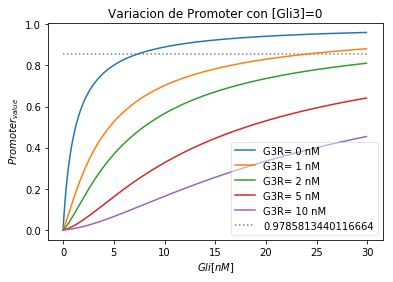
\includegraphics[width=0.8\textwidth]{variacion_promoter}
 	\centering
 	\caption{Variacion del Operador Promoter bajo la variacion de Gli3R }
 	\label{varipro}
 \end{figure}

\begin{figure}[h]
	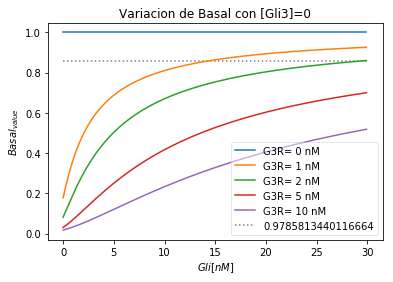
\includegraphics[width=0.8\textwidth]{variacion_basal}
	\centering
	\caption{Variacion del Operador Basal bajo la variación de Gli3R }
	\label{varibas}
\end{figure}

\subsubsection{Reducción de la complejidad del operador}

En los siguientes apartados tendremos que hacer grandes volumenes de cuentas para estudiar variaciones en el comportemiento cualitativo del modelo. Por este motivo cualquier simplificación u optimización es altemente bienvenida a la hora de programar. 

En nuestro caso, basándonos en los resultados de \cite{multiple} tuvimos acceso a una simplificación de los operadores promoter y basal. Antes de realizar el estudio, sin embargo, quisimos comprobar numéricamente la viabilidad frente a multiples variaciones de las dos expresiones. 

Prueba de ello es la figura \ref{compara}, donde mostramos como ambas expresiones son equivalentes cualesquiera variaciones hagamos. Dentro de esta tenemos en color la expresión clásica de los operadores y en líneas discontinuas mostramos la nueva expresion. Como se ve, la coincidencia es perfecta. 

\begin{figure}[h]
	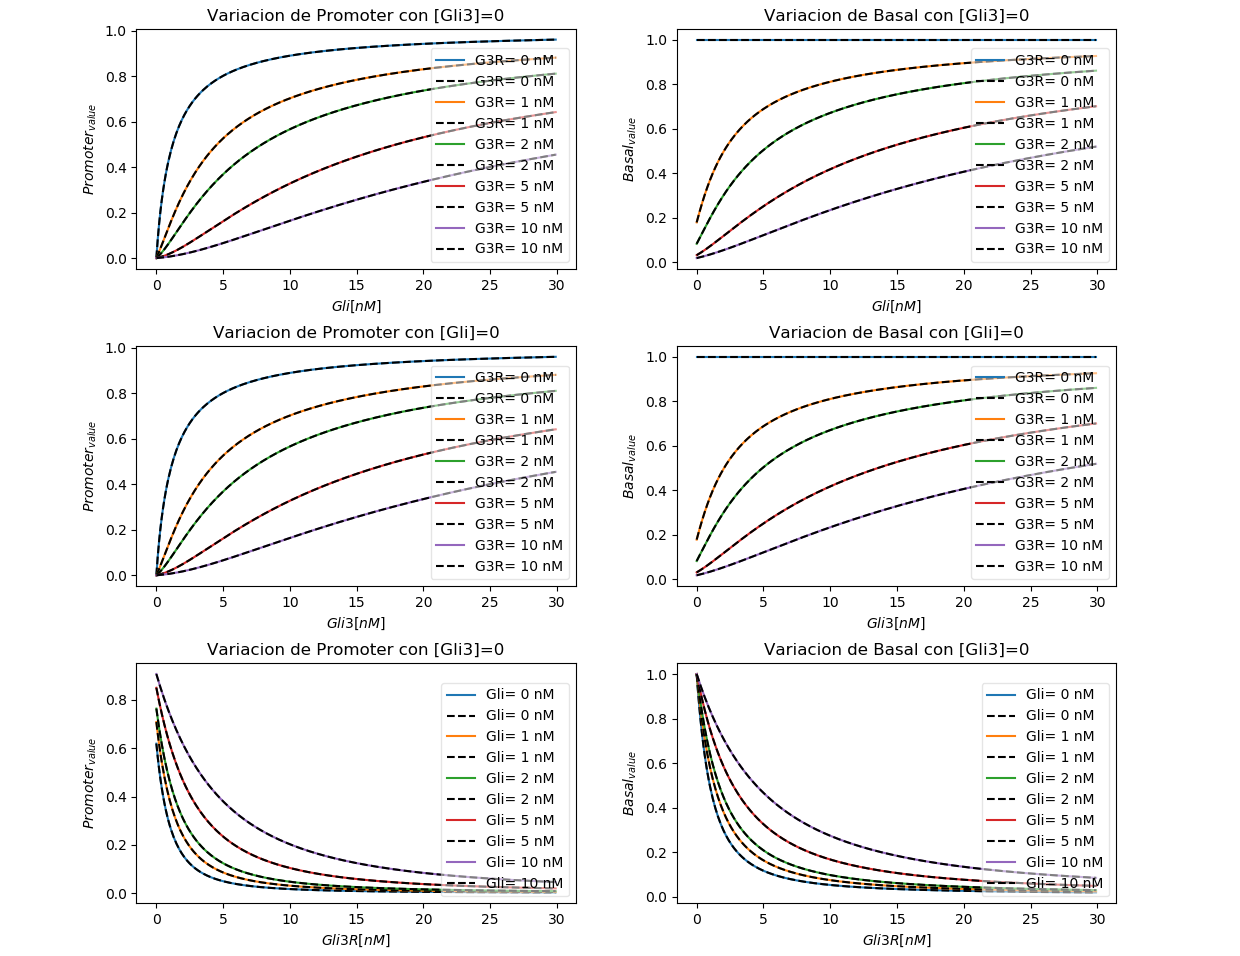
\includegraphics[width=0.8\textwidth]{reduced_form_promoter}
	\centering
	\caption{Comparación numérica de las formas de reducidas de Promoter y Basal (en negro discontinuo) frente a las formas de \cite{schaffer} }
	\label{compara}
\end{figure}

\subsection{Evolución temporal}
Una vez computamos los operadores en su forma reducida, procedimos a simular la evolución temporal del sistema. 

Para ello utilizamos el módulo de cálculo numérico de Python y el algoritmo \textit{lsode} que es robusto frente a comportamientos \textit{stiff}. (Estos cálculos ademas han sido validados y reproducidos con Octave).

En particular corrimos simulaciones con distintas condiciones iniciales y distintos valores de Shh:

\begin{itemize}
	\item Condiciones iniciales: Gli=0.001 $Gli_3$=0 Gli3R=0 Ptc=0.  Valor Shh/$K_{Shh}$: 0,1
	\item Condiciones iniciales: Gli=0.001 $Gli_3$=0 Gli3R=0 Ptc=0.  Valor Shh/$K_{Shh}$: 1,5
	\item Condiciones iniciales: Gli=0.001 $Gli_3$=0 Gli3R=0 Ptc=0.  Valor Shh/$K_{Shh}$: 15
	\item Condiciones iniciales: Gli=1 $Gli_3$=1 Gli3R=1 Ptc=1.  Valor Shh/$K_{Shh}$: 0,1
	\item Condiciones iniciales: Gli=0.001 $Gli_3$=10 Gli3R=10 Ptc=10.  Valor Shh/$K_{Shh}$: 0,1
\end{itemize}

Dentro de estas simulaciones preliminares, en cuanto al estudio cualitativo, observamos dos interesantes comportamientos según varía la cantidad de $Shh/k_{Shh}=0.1$ en \ref{lai1}, $Shh/k_{Shh}=1.5$ en \ref{lai2}. Esto nos confirma la multiestabilidad del sistema que se afirma en el articulo original. Pero, como veremos más adelante, esta debe ser tomada con precaución.

En la Figura \ref{lai1}, podemos observar que si las cantidades de Shh disminuyen en gran medida, tanto Gli como Ptc se van a ver afectados, disminuyendo su cantidad. Esto se debe al aumento de Gli3R en nuestro sistema puesto que el principal inhibidor de la proteólisis de $Gli_3$ en Gli3R es Shh y este se encuentra en baja concentración. 

Por contraparte, en la figura \ref{lai2}, la proporción $Shh/K_{Shh}$ aumenta en gran medida. Esto activa toda la maquinaria bioquímica del proceso, inhibiendo Gli3R, que cae en mínimos y produciendo grandes cantidades de Gli y Ptc.

Los estados estacionarios sirvieron también de punto de partida para nuevas simulaciones, sin embargo, hay resultados de \cite{schaffer} que hemos concluido irreproducibles, destacando la dinámica del sistema con un cambio brusco de la cantidad de Shh\footnote{Figura 2(A) de \cite{schaffer}.}. Por su parte, la dinámica del sistema tampoco se encuentra estudiada, y se presentan en el artículo solo comportamientos de Gli.



 \begin{figure}[h]
 	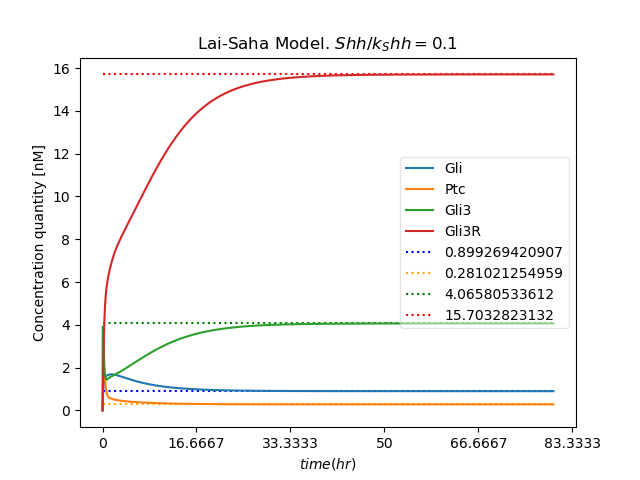
\includegraphics[width=0.8\textwidth]{lai2}
 	\centering
 	\caption{Evolución del modelo \cite{schaffer} con $Shh/k_{Shh}=0.1$ }
 	\label{lai1}
 \end{figure}


\begin{figure}[h]
	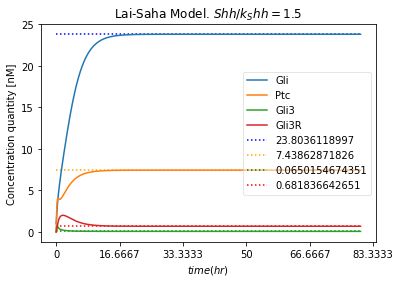
\includegraphics[width=0.8\textwidth]{lai1}
	\centering
	\caption{Evolución del modelo \cite{schaffer} con $Shh/k_{Shh}=1.5$}
	\label{lai2}
\end{figure}

\subsection{Análisis numérico de los estados estacionarios}

Para el análisis numérico de los estados estacionarios seguimos dos estrategias. 
En primer lugar programamos las expresiones analíticas obtenidas en el apartado \ref{apartado2.4}. Con ellas podemos representar la función y la recta $y=Gli$ (tal y como se muestra en la figura \ref{lai_123}). 

Esta representación nos permite observar los puntos de corte de ambas funciones y, con ello inferir los estados estacionarios. Más aun, nos permite observar el comportamiento de la curva más claramente según varían los parámetros para decidir como alterarlos de manera que se produzcan puntos de corte (lo que nos dio una primera intuición sobre $r_{g3b}$).

\begin{figure}[h]
	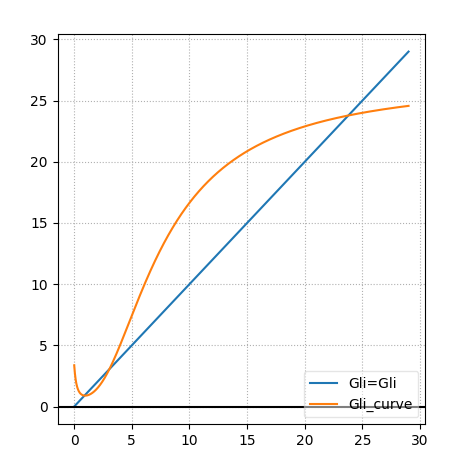
\includegraphics[width=0.5\textwidth]{countingzeroslai}
	\centering
	\caption{Representación gráfica de los puntos de corte entre la recta Gli=Gli y la definida por (\ref{final_gli}).}
	\label{lai_123}
\end{figure}

\begin{figure}[h]
	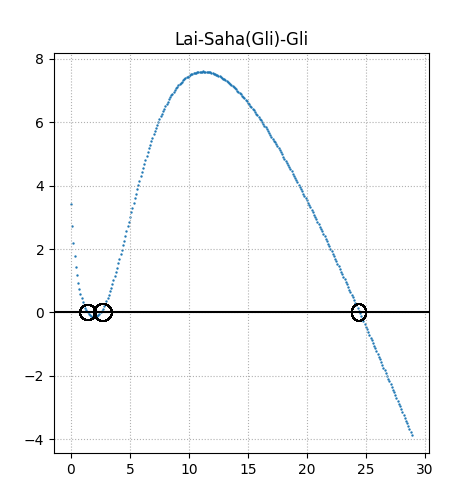
\includegraphics[width=0.5\textwidth]{locatingzeroslai}
	\centering
	\caption{Representación gráfica del procedimiento para buscar ceros implementado. La recta representa la resta entre los miembros de (\ref{final_gli}).}
	\label{lai_124}
\end{figure}


Con esta primera parte, para analizar grandes volúmenes de variaciones de parámetros cambiamos el enfoque. Dado que calculamos de forma discreta, escribimos un programa que computaba la resta de ambas funciones y nos devuelve el número de veces que la resta cambia de signo (es decir, el punto i-ésimo es mayor que cero y el i-esimo +1 es menor, o vicecersa).
El programa produce un \textit{log}, donde se pueden consultar todos los resultados, y guarda en un fichero a parte aquellos que tengan un numero de ceros mayor del configurado.
Extracto del \textit{log} puede verse así:
\begin{verbatim}
Shh = 0.1 r_g3c=1 Zeros:1
\end{verbatim}
En la Figura \ref{lai_124}, se puede observar una representación gráfica de los puntos que buscaría nuestro algoritmo.
Con todo ello, obtivumos intuición sobre que diagramas de bifurcación computar, y obtuvimos el código base para explorar el nuevo modelo.



\subsection{Diagramas de bifurcación}
Durante el estudio de este modelo procedimos también a realizar diagramas de bifurcación\footnote{Un diagrama de bifurcación de un sistema dinámico es una estratificación de su espacio de parámetros inducida por la equivalencia topológica, junto con los retratos de fase representativos de cada estrato.} con aquellos parámetros que el análisis numérico nos mostró como relevantes. Además, procedimos a evaluar la reproducibilidad del artículo en los diagramas que presentan. 

La herramienta escogida para tal fin  fue AUTO, un motor para el cálculo de diagrama de bifurcaciones. En particular utilizamos XppAut, un intérprete de AUTO que nos permite realizar continuación, cambios de ramas y diagramas de bifurcación completos, así como el cálculo de la estabilidad de los puntos fijos. 

Para una mayor profundización en el análisis numérico de bifurcaciones puede consultarse \cite{meijer2012numerical}. Además, en mi trabajo de fin de grado \cite{Yo} puede encontrarse una guía básica de AUTO para interpretar los resultados que imprime por pantalla (se maneja desde la terminal) y como pasarlos a un diagrama. Señalamos que la generación de diagramas de bifurcación es un tema denso y de alta sensibilidad numérica, por lo que recomendamos visitar los dos documentos citados. 

Exponemos también, brevemente la técnica empleada para la obtención:
\begin{enumerate}
	\item Comenzamos utilizando estados cercanos a los estados estacionarios como punto de partida para la iteración temporal\footnote{Es importante señalar que la interación temporal usa un jacobiano calculado por la máquina, no introducido manualmente (pues AUTO ofrece esta posibilidad)}.
	\item Posteriormente a la iteración en tiempo, alcanzamos un valor estacionario con una sensibilidad previamente introducida a la máquina.
	\item Utilizamos XppAut para obtener la estabilidad de la solución obtenida. En caso de ser estable, procedemos a exportar el resultado a AUTO, donde generaremos el diagrama.
	\item En AUTO ajustamos los parámetros numéricos del programa. En particular el tamaño de paso (positivo para generar ramas según aumenta el parámetro y negativo para hacerlo según disminuye ).
	\item Podemos adecuar también el salto entre las ramas del diagrama para englobar posibles comportamientos extraños.
	\item Finalmente generamos un archivo AUTO con la información del diagrama y, inmediatamente después, el diagrama. 
\end{enumerate} 

\subsubsection{Bifurcación bajo $Shh/K_{Shh}$}
Debido a las diferencias que pudimos encontrar durante el desarrollo del modelo, nos pareció interesante intentar reproducir el comportamiento de Gli frente a la variación de $Shh/K_{Shh}$.  En la figura \ref{lai_12} se puede encontrar el diagrama hallado. En ese caso las líneas rojas representan estados estables y las negras inestables. 

En este caso, frente a los resultados del paper, obtenemos un comportamiento de interruptor biestable, sin embargo este no es reversible si no irreversible\footnote{Esta denominación es la elegida por los autores del artículo para denominar aquel comportamiento biestable que no puede cambiar entre estados.}. Es este mismo hecho el que motiva que las líneas del diagrama sobrpasen el 0 para valores de Shh cuando estamos retrocediendo.

Estos resultados, aunque muestran una dinámica similar, difieren cualitativamente de \cite{schaffer}. Sin embargo una revisión bibliográfica nos mostró como se relacionan con los posteriores trabajos del equipo, en concreto \cite{saha}. 

Tendremos, a vista del diagrama, una fuerte rama estable en creciente hacia los 25nmol de Gli y, podemos encontrar otro estado estable con una menor cantidad de Gli según crece la cantidad de Shh hacia 1,8. Es de esperar que Gli acabe cayendo en la región estable superior.

\begin{figure}[h]
	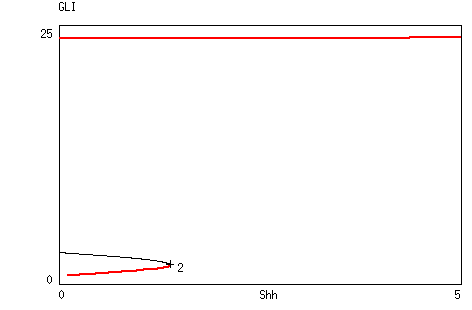
\includegraphics[width=0.8\textwidth]{diagramaweno1}
	\centering
	\caption{Diagrama de Bifurcación de \cite{schaffer} con $Gli$ frente a $Shh/K_{Shh}$}
	\label{lai_12}
\end{figure}



\subsubsection{Bifurcación bajo $r_{g3b}$}
Durante el desarrollo de los estados estacionarios, pudimos observar como las variaciones en la tasa de sintetización basal del $Gli_3$ afectaban dramáticamente a los puntos de corte.

 Con ello, teniendo como referencia los códigos del apéndice \ref{ch:app}, desarrollamos el diagrama de bifurcaciones de Gli frente al a variación de este parámetro  en la figura \ref{lai_2}, algo que no tenemos constancia de que se hubiese llevado a cabo.

 En general, concluimos que la tasa de generación de $Gli_3$ juega un papel fundamental en la dinámica de este modelo, tanto por su posible alteración escogiendo como elemento delimitante Gli o Ptc, como por la variación de este en sí misma. 
 
\begin{figure}[h]
	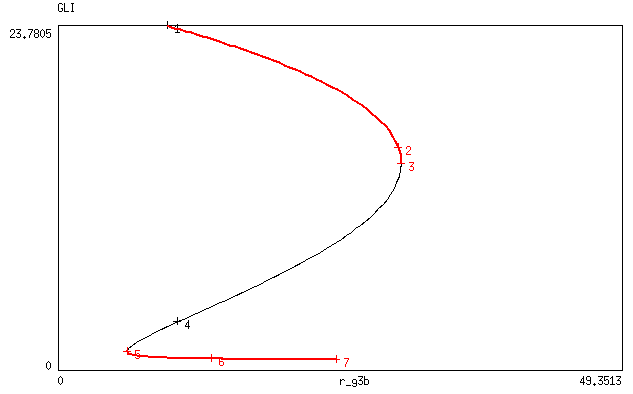
\includegraphics[width=0.8\textwidth]{gliVSr_g3b}
	\centering
	\caption{Diagrama de Bifurcación de \cite{schaffer} con $Gli$ frente a $r_{g3b}$}
	\label{lai_2}
\end{figure}

\section{Críticas}
Aunque el modelo es un referente desde hace muchos años, hemos encontrado dificultades a la hora de estudiarlo. Exponemos una breve crítica al mismo de carácter constructivo.
\begin{itemize}
	\item Posibles erratas: Si bien el comportamiento es el esperado y descrito en la mayoría de los casos, ha sido habitual durante la investigación encontrarnos con problemas a la hora de reproducir los resultados que vienen descritos en el articulo. 
	La ausencia de datos abiertos para esta tarea, la ausencia del código usado en muchos casos y, de código privativo en otros, dificulta en gran medida el estudio y reproducción. Dejamos patente que hay gráficas (corregidas en otros artículos) y expresiones con algunas erratas que pueden llevar a error.
	
	\item Algunas simplificaciones del modelo necesarias para el desarrollo del mismo pueden ser atacadas para estudiarlo en más profundidad. En particular, es nuestro enfoque añadir detalles que este modelo no contempla con el fin de estudiar si así podemos comprender mejor este proceso. 
\end{itemize}



